% Autor: Leonhard Segger, Alexander Neuwirth
% Datum: 2017-10-30
\documentclass[
	% Papierformat
	a4paper,
	% Schriftgröße (beliebige Größen mit „fontsize=Xpt“)
	12pt,
	% Schreibt die Papiergröße korrekt ins Ausgabedokument
	pagesize,
	% Sprache für z.B. Babel
	ngerman
]{scrartcl}

% Achtung: Die Reihenfolge der Pakete kann (leider) wichtig sein!
% Insbesondere sollten (so wie hier) babel, fontenc und inputenc (in dieser
% Reihenfolge) als Erstes und hyperref und cleveref (Reihenfolge auch hier
% beachten) als Letztes geladen werden!

\usepackage{tikz}
\usetikzlibrary{calc,patterns,angles,quotes} % loads some tikz extensions\usepackage{tikz}
\usetikzlibrary{babel}

% Silbentrennung etc.; Sprache wird durch Option bei \documentclass festgelegt
\usepackage{babel}
% Verwendung der Zeichentabelle T1 (Sonderzeichen etc.)
\usepackage[T1]{fontenc}
% Legt die Zeichenkodierung der Eingabedatei fest, z.B. UTF-8
\usepackage[utf8]{inputenc}
% Schriftart
\usepackage{lmodern}
% Zusätzliche Sonderzeichen
\usepackage{textcomp}

% Mathepaket (intlimits: Grenzen über/unter Integralzeichen)
\usepackage[intlimits]{amsmath}
% Ermöglicht die Nutzung von \SI{Zahl}{Einheit} u.a.
\usepackage{siunitx}
% Zum flexiblen Einbinden von Grafiken (\includegraphics)
\usepackage{graphicx}
% Abbildungen im Fließtext
\usepackage{wrapfig}
% Abbildungen nebeneinander (subfigure, subtable)
\usepackage{subcaption}
% Funktionen für Anführungszeichen
\usepackage{csquotes}
\MakeOuterQuote{"}
% Zitieren, Bibliografie
\usepackage[sorting=none]{biblatex}


% Zur Darstellung von Webadressen
\usepackage{url}
%chemische Formeln
\usepackage[version=4]{mhchem}
% siunitx: Deutsche Ausgabe, Messfehler getrennt mit ± ausgeben
\usepackage{floatrow}
\floatsetup[table]{capposition=top}
\usepackage{float}
% Verlinkt Textstellen im PDF-Dokument
\usepackage[unicode]{hyperref}
% "Schlaue" Referenzen (nach hyperref laden!)
\usepackage{cleveref}
\sisetup{
	locale=DE,
	separate-uncertainty
}
%\bibliography{6Mi_M3_29-11-2017_References}
%TODO anpassen

\begin{document}

	\begin{titlepage}
		\centering
		{\scshape\LARGE Versuchsbericht zu \par}
		\vspace{1cm}
		{\scshape\huge V06 - $\beta$-Zerfall \par} %TODO Anpasen
		\vspace{2.5cm}
		{\LARGE Gruppe BA-C-04 \par}
		\vspace{0.5cm}

		{\large Alexander Neuwirth (E-Mail: a\_neuw01@wwu.de) \par}
		{\large Leonhard Segger (E-Mail: l\_segg03@uni-muenster.de) \par}
		\vfill

		durchgeführt am 29.04.2019\par %TODO Anpassen
		betreut von\par
		{\large Lucia Anna Husová} %TODO Anpassen

		\vfill

		{\large \today\par}
	\end{titlepage}
	\tableofcontents
	\newpage

	%TODO mehr TODO in Default

	\section{Kurzfassung}
	% Hypothese	und deren Ergebnis, wenn Hypothese ist, dass nur Theorie erfüllt, sagen: Erwartung: Theorie aus einführung (mit reflink) erfüllt
	% Ergebnisse, auch Zahlen, mindestens wenn's halbwegs Sinn ergibt
	% Was wurde gemacht
	% manche leute wollen Passiv oder "man", manche nicht

  \section{Theorie}
	% wdh. Texte
	% wdh. Besprechung

	\begin{equation}
		B\rho = \sqrt{\frac{E_k^2+2E_kmc^2}{c^2e^2}}
	\end{equation}

	\section{Methoden}
	% Bilder von der Website klauen
	% einer will Präsens

	\section{Ergebnisse und Diskussion}
	%TODO Unsicherheiten


	\subsection{Beobachtung und Datenanalyse}
	% Allgemeine Beobachtungen
	% Einflüsse von veränderten Parametern auf Messung
	%\subsubsection{Unsicherheiten}
	% Berechung nach Aufgabenstellung
	\subsubsection{Untergrund}
	In \cref{fg_untergrund} sind die gemessenen Ereignisraten gegen die angelegte Spannungen aufgetragen.
	Die blaue Horizontale ist jeweils an einen Bereich von \SI{0.25}{V} am Anfang und Ende der Messkurve angepasst und beschreibt so die Untergrundrate.
	\begin{figure}[H]
			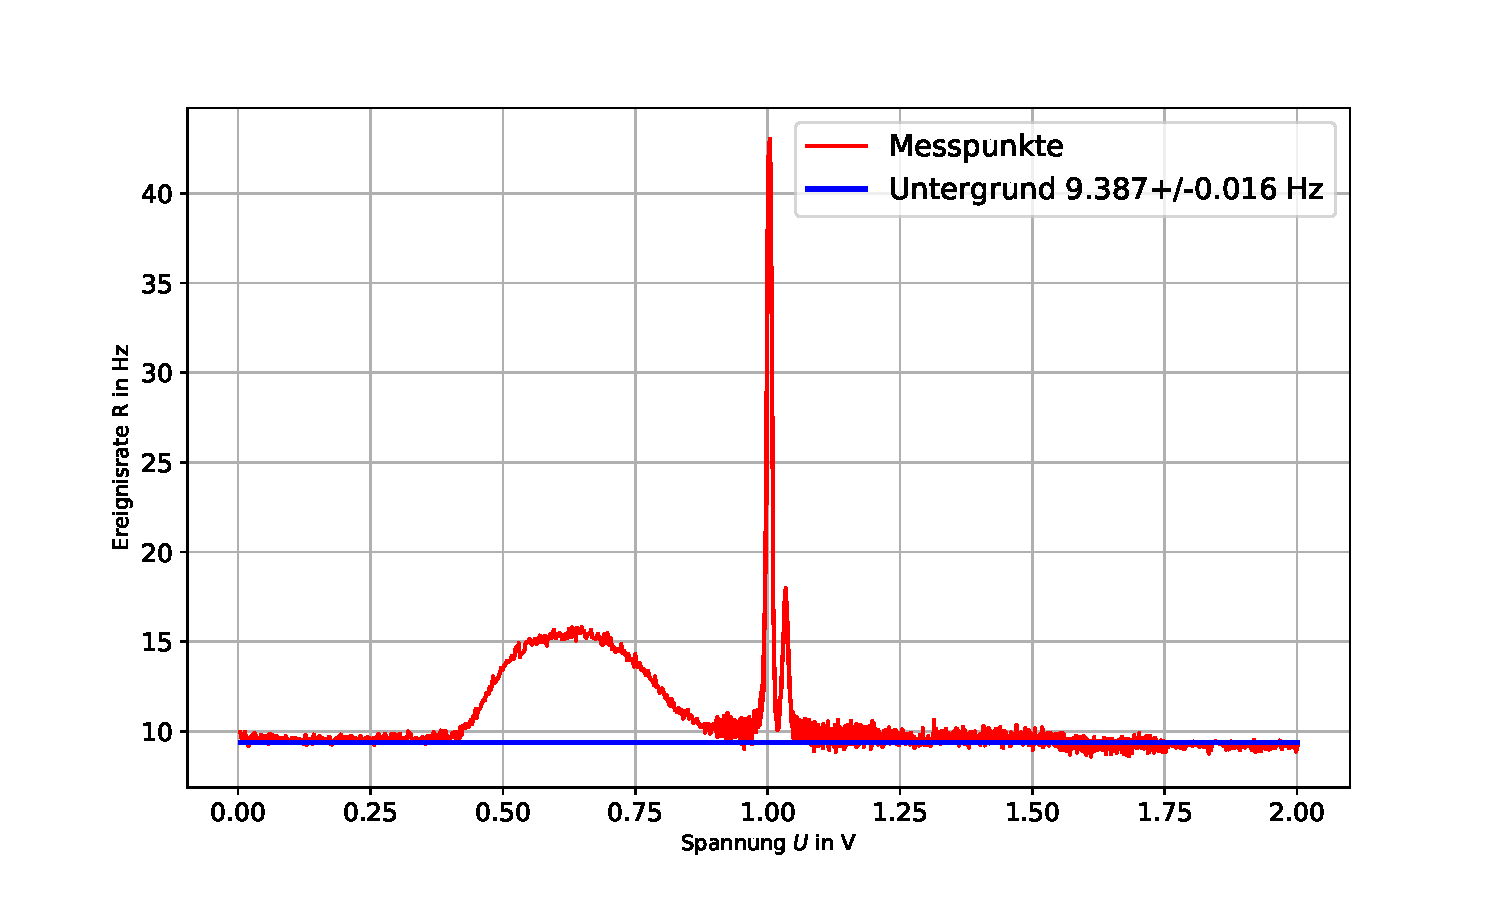
\includegraphics[width=  \linewidth]{img/untergrund}
			\caption{
			Die Anzahl der Ereignisse wurde durch die Messzeit bei einer festen Spannung dividiert, sodass sich die Ereignisrate ergibt.
			Die Unsicherheiten sind kleiner als die Symbole.
			}
			\label{fg_untergrund}
	\end{figure}

	\subsubsection{Kalibration des Spektrometers}
	Um das Spektrometer zu Kalibrieren nutzt man, dass die Konversionselektronen des $^{137}$Ba eine scharfe Energie haben.
	Diese Energien sind bekannt und in \cref{tb_konversion} aufgelistet.
	Dabei ist der Wert für die L-Linie der nach den Intensitäten der drei L-Linien gewichtete Mittelwert.

\begin{table}[H]
		\centering
		\begin{tabular}{c | c | c  }
			 Schale&E in \si{keV} & $B\rho$ in \si{Tcm} \\ \hline
			 K & \SI{624.21}{} & \SI{0.33814(5)}{} \\
			 L & \SI{655.8}{} & \SI{0.3499(1)}{} \\
		\end{tabular}
		\caption{
		Gemittelte Energie der L und K Konversionselektronen von $^{137}$Ba und zugehöriger B$\rho$-Wert. \cite{Anleitung}
		}
		\label{tb_konversion}
\end{table}
In \cref{fg_kalibration} sind die zwei Peaks vergrößert dargestellt und es wurden jeweils die Spitzen mit einer Gaußfunktion angepasst.
Außerdem wurde der zuvor bestimmte Untergrund subtrahiert.
	\begin{figure}[H]
			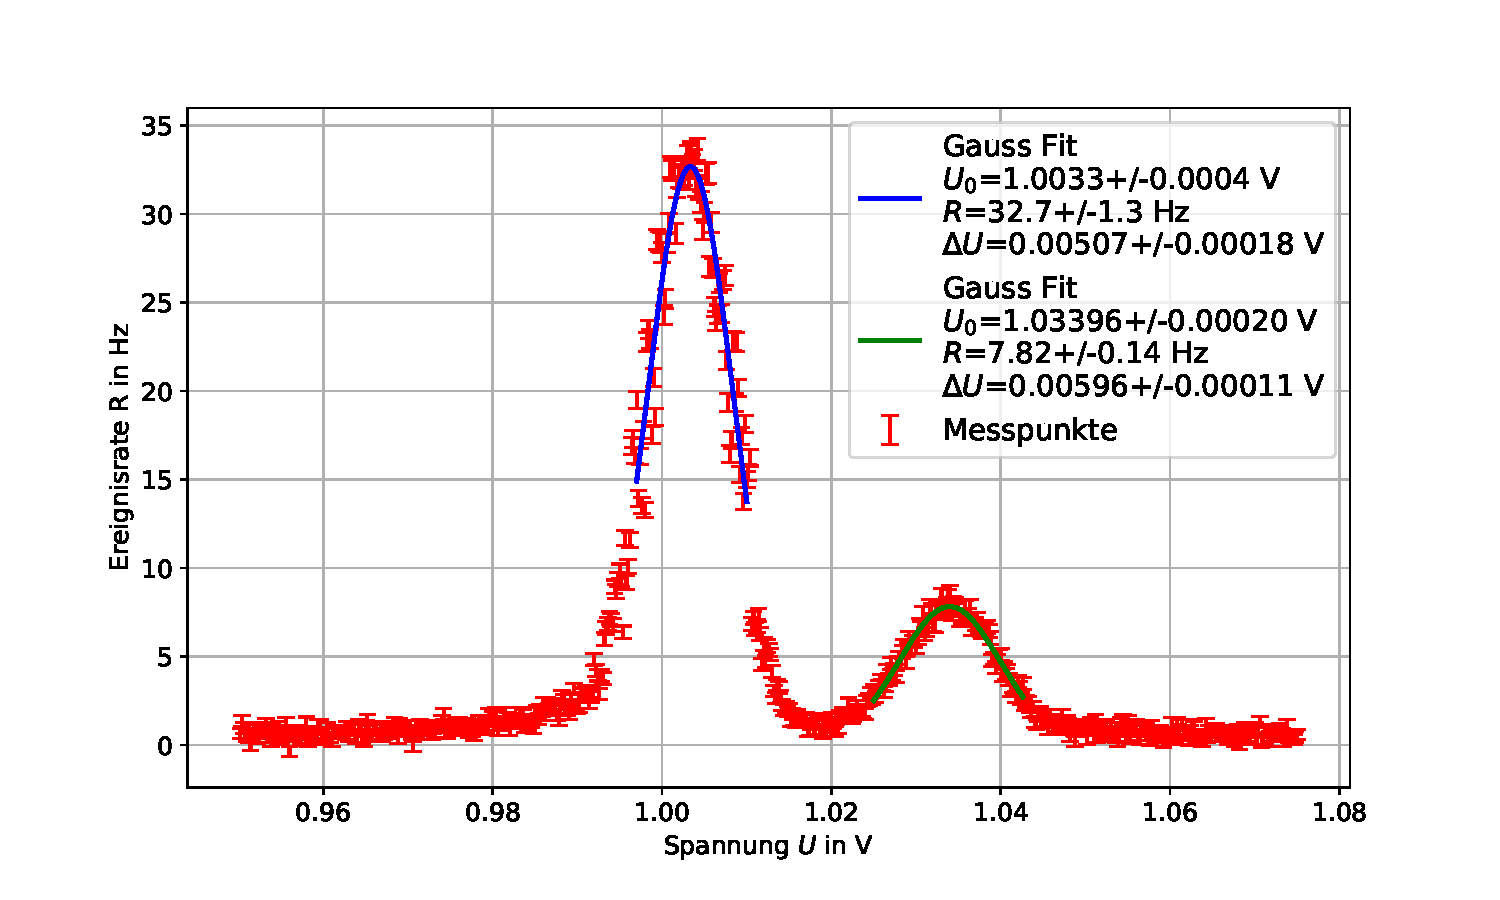
\includegraphics[width=  \linewidth]{img/kalibration}
			\caption{
			Vergrößerte und um den Untergrund reduzierte Messung der Peaks.
			Der größere Peak ist der K-Peak.
			Die Unsicherheiten sind kleiner als die Symbole.
			}
			\label{fg_kalibration}
	\end{figure}

	Da mit einem Magnetspektrometer jedoch ein Impuls $p=eB\rho$ anstelle einer Energie gemessen wird, kalibriert man zunächst nach $B\rho$.
	Der Kalibrationsparameter ergibt sich aus dem Verhältnis von der Differenz der $B\rho$-Werte und dem Abstand der Peaks.
	\begin{equation}
		a = \frac{\Delta B\rho}{\Delta U} = \frac{\SI{0.0118+-0.0001}{Tcm}}{\SI{0.031+-0.007}{V}} = \SI{0.384+-0.089}{Tcm/V}
	\end{equation}
	Für die Unsicherheit der Peakpositionen wurde die Breite des Gaußfits verwendet.
	Die gemäß \cref{eq_rho} kalibrierte Messkurve ist in \cref{fg_kali} enthalten.
	\begin{equation}
		\label{eq_rho}
		B\rho = aU-aU_{0,K}+(B\rho)_K
	\end{equation}
	\begin{figure}[H]
			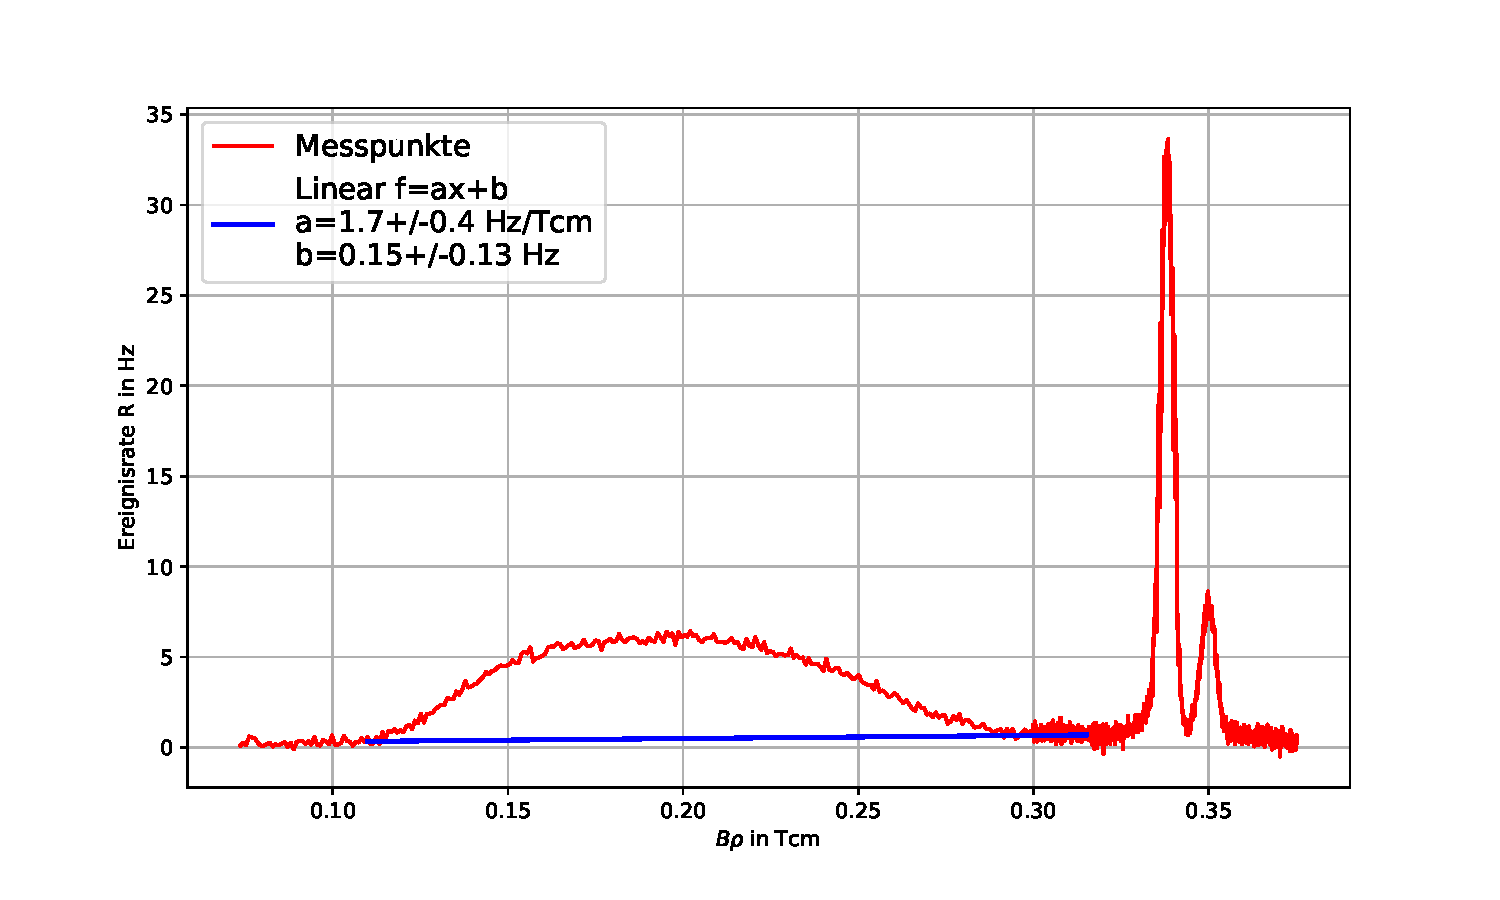
\includegraphics[width=  \linewidth]{img/kali}
			\caption{
			Um den Untergrund und Ränder reduzierte kalibrierte Messung.
			Die Unsicherheiten sind kleiner als die Symbole.
			}
			\label{fg_kali}
	\end{figure}
	Für die Impulsauflösung folgt:
	\begin{equation}
		R = \frac{\Delta B \rho}{B\rho} = \frac{2\sqrt{2\ln2}a\Delta U}{aU-aU_{0,K}+(B\rho)_K}
	\end{equation}
	Der Faktor $2\sqrt{2\ln2}$ kommt daher, dass $\Delta U$ die Standardabweichung der Gaußkurve ist, die Definition der Impulsauflösung aber $\Delta B\rho$ als Halbwertsbreite verlangt.
	Für die zwei Peaks ergibt sich:
	\begin{align}
	R_K&= \SI{14+- 0.3}{\percent} \\
	R_L&= \SI{16+-0.4}{\percent}
	\end{align}
	\subsection{Diskussion}
	% Bezug/Nutzen oder sonst was
	% auch hier die Hypothese wiederholen
	% keine Messwerte hier, nach manchen Menschen, zumindest "direkt" erstellte Diagramme net hier, auch wenn Lesbarkeit-bla

	%TODO gewisserweise erwartet, dass die Impulsauflösung weiter entfernt von dem Kalibrierpunkt schlechter wird.

	\section{Schlussfolgerung}
	% Rückgriff auf Hypothese und drittes Nennen dieser

	% Quellen zitieren, Websiten mit Zugriffsdatum
	% Verweise auf das Laborbuch (sind erlaubt)
	% Tabelle + Bilder mit Beschriftung
	%\printbibliography
\end{document}
